
 \subsection{Regressão logística}
 A regressão logística é um método estatístico utilizado para modelar a probabilidade de uma variável 
dependente categórica. É comumente utilizada para problemas de classificação binária, onde a variável
dependente possui apenas duas categorias, como sim/não, positivo/negativo, 0/1.

% TODO: melhorar isso
% falar direto da equação 8.1.2,

O cálculo da regressão logística é baseado na probabilidade da variável aleatória $Y$ ser igual a 1, onde Y é 
uma variável aleatória com distribuição Bernouli, com parâmetro p de sucesso, cuja fórmula é dada por:

\begin{equation}
  P(Y=1| X_1, X_2, ..., X_k) = \frac{1}{1 + e^{-(\beta_0 + X_{1}\beta_1 + X_{2}\beta_2 + \ldots +X_{k}\beta_k)}}
\end{equation}

\noindent onde cada variável explicativa $(X_1, X_2, ..., X_k)$ tem um parâmetro $\beta$ correspondente, influenciando o resultado de $Y$.

A estimação dos coeficientes $(b_0, b_1, b_2, ..., b_k)$  na regressão logística é geralmente realizada por meio 
do método da máxima verossimilhança. O objetivo é encontrar os valores dos coeficientes que maximizam a função de
verossimilhança, representando a probabilidade de observar os dados observados dado o modelo.
 
A função de verossimilhança $(L)$ para a regressão logística é dada pelo produto das probabilidades condicionais
de observar os eventos(valores da variável dependente) dados os valores das variáveis independentes. Para facilitar o cálculo, 
geralmente trabalhamos com o logaritmo natural da função de verossimilhança, conhecido como log-verossimilhança($l$).

A log-verossimilhança para a regressão logística é:

\begin{equation}
  l(\beta) = \sum_{i=1}^{N} [y_i \beta^T x_i - \log(1 + e^{\beta^T x_i})]
\end{equation}


\begin{itemize}
  \item  $N$é o número total de observações.
  \item  $y_i$ é a variável dependente binária da i-ésima observação (0 ou 1).
  \item $p_i$ é a probabilidade predita de $Y=1$ para a i-ésima observação, dada pela função logística.
\end{itemize}

A ideia é encontrar os valores de $(b_0, b_1, b_2, ..., b_k)$ que maximizam essa função. Isso geralmente é feito usando métodos computacionais, 
como o algoritmo de otimização Newton-Raphson ou o Gradiente Descendente.

Para se interpretar o modelo logístico é utilizado o método da Razão de Chances, que calcula a razão da
probabilidade de um evento ocorrer em um grupo em relação à probabilidade de não ocorrer. 

Esse resultado pode ser obtido quando se calcula a exponencial dos coeficientes do modelo logístico.

\begin{equation}
  RC = \exp{(\beta_k)}
\end{equation}

Um RC igual a 1 indica que a variável independente não tem efeito no resultado de Y(nenhuma associação).
Um RC maior que 1 sugere uma associação positiva, enquanto um RC menor que 1 sugere uma associação negativa.

Outra medida interpretativa é a função log odds ou logíto. Ela é uma função que calcula o log da 
razão do evento acontecer e dele não acontecer, cuja formulação é dada por:

\begin{equation}
  \text{logit}(P(Y=1)) = \log \left( \frac{P(Y=1)}{1 - P(Y=1)} \right)
\end{equation}

Onde esse resultado nada mais é do que $\beta_0 + X_{1}\beta_1 + X_{2}\beta_2 + \ldots +X_{k}\beta_k$. 

Portanto, a utilidade de se analisar o log-odds é justamente uma ponte entre olhar coeficiente e a probabilidade final, 
pois um coeficiente positivo indica que o aumento na variável está associado a um aumento nas log-odds 
(e, portanto, na probabilidade), enquanto um coeficiente negativo está associado a uma diminuição nas log-odds (e na probabilidade).


\subsection{Métricas de avaliação}

A avaliação do desempenho dos modelos é fundamental para obter insights sobre sua eficácia nas predições ou classificações. 
A utilização de estratégias que resumem o desempenho por meio de métricas específicas é crucial nesse processo.
A análise dessas métricas proporciona uma compreensão mais aprofundada do modelo, permitindo identificar pontos 
fortes e áreas de melhoria. Essa avaliação não apenas valida a qualidade das previsões, mas também orienta os próximos
passos na pesquisa, direcionando ajustes necessários no modelo ou indicando caminhos para refinamento. 
Dessa forma, a escolha e interpretação adequadas das métricas são passos essenciais para uma avaliação informada 
e um progresso significativo na pesquisa.

\subsubsection{Matriz de confusão}

Uma matriz de confusão é uma tabela usada para avaliar o desempenho de um modelo de classificação.
Seu papel é de expor os resultados das predições do modelo quando comparadas com os valores reais.

A matriz de confusão organiza as previsões do modelo em quatro categorias, comumente chamadas de Verdadeiro Positivo (VP), 
Falso Positivo (FP), Verdadeiro Negativo (VN) e Falso Negativo (FN). Essas categorias são definidas da seguinte maneira:

\begin{itemize}
  \item Verdadeiro Positivo (VP): Exemplos que foram corretamente classificadas como pertencentes à classe positiva.
  \item Falso Positivo (FP): Exemplos que foram erroneamente classificadas como pertencentes à classe positiva, quando na verdade pertencem à classe negativa.
  \item Verdadeiro Negativo (VN): Exemplos que foram corretamente classificadas como pertencentes à classe negativa. 
  \item Falso Negativo (FN): Exemplos que foram erroneamente classificadas como pertencentes à classe negativa, quando na verdade pertencem à classe positiva.
\end{itemize}

\begin{table}[h]
  \centering
  \begin{tabular}{c|c|c|c|}
  & & \multicolumn{2}{c|}{\textbf{Previsão}} \\ \cline{3-4}
  & & \textbf{Positivo} & \textbf{Negativo} \\ \hline
  \multicolumn{1}{|c|}{\multirow{2}{*}{\textbf{Real}}} & \textbf{Positivo} & Verdadeiro Positivo (VP) & Falso Negativo (FN) \\ \cline{2-4}
  \multicolumn{1}{|c|}{} & \textbf{Negativo} & Falso Positivo (FP) & Verdadeiro Negativo (VN) \\ \hline
  \end{tabular}
  \caption{Matriz de Confusão}
  \label{table:confusion_matrix}
\end{table}

\subsubsection{Acurácia}
A acurácia é a proporção de predições corretas feitas por um modelo em relação ao número total de predições. 
A fórmula básica para calcular a acurácia é dada por:

\begin{equation}
  \text{Acurácia} = \frac{\text{Número de predições corretas}}{\text{Número total de predições}} = \frac{VP+VN}{VP+VN+FP+FN}
\end{equation}

Essa métrica fornece uma visão geral do desempenho do modelo, indicando a porcentagem de instâncias corretamente classificadas.
No entanto, a acurácia pode ser enganosa em casos onde as classes não estão balanceadas. 
Em situações desse tipo, um modelo que prevê sempre a classe majoritária pode ter uma acurácia alta, mesmo que não seja eficaz.

\subsubsection{Precisão}

A precisão é definida como a proporção de exemplos classificados corretamente como positivos em 
relação ao total de exemplos classificadas como positivas (verdadeiras positivas mais falsos positivos).

\begin{equation}
  \text{Precisão} = \frac{VP}{VP + FP}
\end{equation}

A precisão é particularmente útil quando os falsos positivos são mais problemáticos ou custosos
em comparação com os falsos negativos. Por exemplo, em um sistema de detecção de spam, classificar 
erroneamente um e-mail legítimo como spam (falso positivo) pode ser mais prejudicial do que deixar
passar um e-mail de spam (falso negativo).

\subsubsection{Recall}

O recall, também conhecido como sensibilidade, é outra métrica utilizada no contexto de classificação, 
focada em capturar a proporção de exemplos positivos que foram corretamente identificadas pelo modelo
em relação ao total de exemplos positivos existentes.

\begin{equation}
  \text{Recall} = \frac{VP}{VP + FN}
\end{equation}

O recall é especialmente útil quando os falsos negativos (exemplos positivos não identificadas pelo modelo) 
são mais críticos ou custosos do que os falsos positivos. Por exemplo, em um sistema de detecção de fraudes,
é crucial identificar todas as transações fraudulentas, mesmo que isso signifique aceitar algumas transações 
normais erroneamente classificadas como fraudulentas.


\subsubsection{F1-score}

O F1-score é uma métrica de avaliação que combina as métricas de precisão e recall em um único valor. 

\begin{equation}
  F1 = 2 \cdot \frac{\text{Precisão} \cdot \text{Recall}}{\text{Precisão} + \text{Recall}}
\end{equation}

O F1-score é a média harmônica entre a precisão e o recall. A média harmônica é utilizada porque penaliza extremos, 
sendo particularmente sensível a baixos valores em qualquer uma das métricas.

O F1-score varia de 0 a 1, onde 1 indica o melhor desempenho possível, equilibrando tanto a precisão quanto o recall.
Essa métrica é particularmente útil quando há um desequilíbrio significativo entre as classes, 
pois é menos sensível a grandes quantidades de verdadeiros negativos.


\subsection{Redes neurais artificiais}

Redes Neurais Artificiais (ou \textit{Deep Learning}) é uma técnica preditiva presente no campo de Inteligência Artificial. As redes neurais tem sido amplamente utilizadas devido ao seu alto poder preditivo e também à flexibilidade de se aplicar esse método em diversos contextos, permitindo ser um modelo com menos restrições que os modelos tradicionais estatísticos.


\subsubsection{Neurônio}

Uma rede neural tem esse nome devido à tentativa de se reproduzir o comportamento do cérebro humano. Sua arquitetura é composta por um conjunto de unidades denominadas neurônios, e cada neurônio é responsável por receber informações, fazer o tratamento do que foi recebido, e repassar o resultado disso para frente. A Figura \ref{neuronio} ilustra a estrutura de 1 neurônio. Quando as informações $x_i$ entram no neurônio, acontece primeiramente um processo onde é ponderada cada informação que foi recebida, os chamados \textbf{pesos}. Logo em seguida ocorre a soma dessa ponderação. Feito isso, é realizado mais um processo de soma, agora adicionando uma informação própria daquele neurônio nesse resultado. Essa informação é chamada de \textbf{bias} (ou Viés). Antes desse resultado ser repassado para outro neurônio, ele passa por uma função que vai definir a natureza daquela informação, chamada de \textbf{função de ativação}, retornando assim uma saída $y$.

 \begin{figure}[H]
    \centering
     \caption{Neurônio da Rede Neural}
    \begin{tikzpicture}[
init/.style={
  draw,
  circle,
  inner sep=2pt,
  font=\Huge,
  join = by -latex
},
squa/.style={
  draw,
  inner sep=2pt,
  font=\Large,
  join = by -latex
},
start chain=2,node distance=13mm,
scale = 0.6
]
\node[on chain=2] 
  (x2) {$x_2$};
\node[on chain=2,join=by o-latex] 
  {$w_2$};
\node[on chain=2,init] (sigma) 
  {$\displaystyle\Sigma$};
\node[on chain=2,squa,label=above:{\parbox{2cm}{\centering Função de Ativação}}]   
  {$f$};
\node[on chain=2,label=above:Saída,join=by -latex] 
  {$y$};
\begin{scope}[start chain=1]
\node[on chain=1] at (0,1.5cm) 
  (x1) {$x_1$};
\node[on chain=1,join=by o-latex] 
  (w1) {$w_1$};
\end{scope}
\begin{scope}[start chain=3]
\node[on chain=3] at (0,-1.5cm) 
  (x3) {$x_3$};
\node[on chain=3,label=below:Pesos,join=by o-latex] 
  (w3) {$w_3$};
\end{scope}
\node[label=above:\parbox{2cm}{\centering Viés \\ $b$}] at (sigma|-w1) (b) {};

\draw[-latex] (w1) -- (sigma);
\draw[-latex] (w3) -- (sigma);
\draw[o-latex] (b) -- (sigma);

\draw[decorate,decoration={brace,mirror}] (x1.north west) -- node[left=10pt] {Entradas} (x3.south west);
\end{tikzpicture}
   
    \label{fig:my_label}
\end{figure} 

A Figura \ref{fig:my_label} pode ser representada matematicamente da seguinte maneira:
\begin{equation}
    y = f (\beta + \sum_{i=1}^{d_x} w_ix_{i} ) 
    \label{neuronio}
\end{equation}
 
 onde $d_x$ é o número de entradas.


\begin{figure}[H]
    \centering
    \caption{Tipos de Função de Ativação.}
    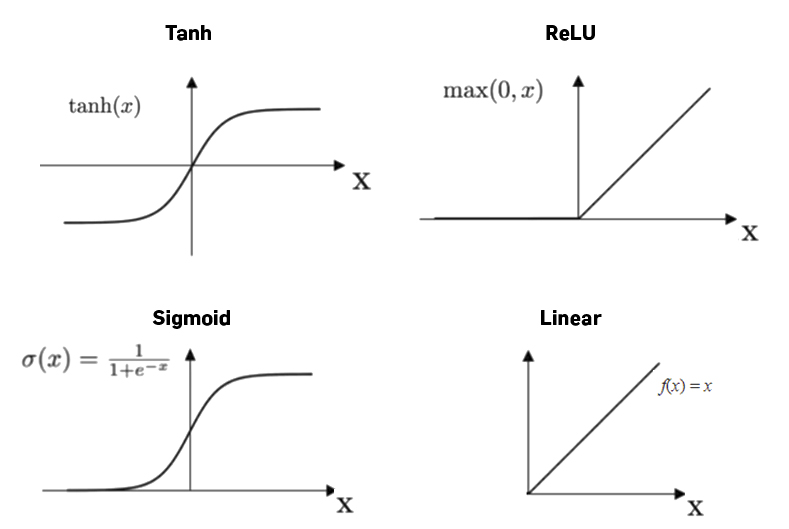
\includegraphics[scale=0.4]{imagens/activation-functions3.jpg}
    \caption*{Fonte: https://machine-learning.paperspace.com/wiki/activation-function}
    \label{fig:func_ativac}
    
\end{figure}

A Figura \ref{fig:func_ativac} mostra alguns tipos de funções de ativação que um neurônio pode ser atribuído. Note como a maioria dessas funções restringe o valor de x (nesse caso o valor calculado no neurônio), no caso da função Sigmoide e da Tangente hiperbólica (tanh) limitando o valor do neurônio em um intervalo, a ReLU, que é bastante utilizada, desconsidera os valores negativos e existe a função Linear que basicamente só vai repassar a informação do neurônio para frente.

\vspace{1cm}



\subsubsection{Arquitetura}

Uma rede neural é estruturada em camadas formadas por um conjunto de neurônios. Conforme ilustrado na Figura \ref{fig:arc_smp_rnp}, temos as camadas de entrada, as camadas ocultas e a camada de saída. A camada de entrada é o ponto de partida da rede neural, pois é onde as informações das variáveis entram. Logo em seguida encontram-se as camadas ocultas, que são as principais responsáveis por criar redes mais complexas, pois o número de camadas e o número de neurônio dentro dessas camadas podem ser moldados ou adicionados dependendo do objetivo empregado pela rede, conforme ilustrado na Figura \ref{fig:arc_cpx_rnp}. E por fim existe a camada de saída que contém o(s) valor(es) predito(s) pela rede.

\begin{figure}[H]
\centering
\caption{Rede Neural com uma camada oculta}
\begin{tikzpicture}[
plain/.style={
  draw=none,
  fill=none,
  },
net/.style={
  matrix of nodes,
  nodes={
    draw,
    circle,
    inner sep=10pt
    },
  nodes in empty cells,
  column sep=2cm,
  row sep=-9pt
  },
>=latex
]
\matrix[net] (mat)
{
|[plain]| \parbox{1.3cm}{\centering Camada \\Entrada} & |[plain]| \parbox{1.3cm}{\centering Camada\\Oculta} & |[plain]| \parbox{1.3cm}{\centering Camada\\Saída}\\
& |[plain]| \\
|[plain]| & \\
& |[plain]| \\
  |[plain]| & |[plain]| \\
& & \\
  |[plain]| & |[plain]| \\
& |[plain]| \\
  |[plain]| & \\
& |[plain]| \\    };
\foreach \ai [count=\mi ]in {2,4,...,10}
  \draw[<-] (mat-\ai-1) -- node[above] {Entrada \mi } + (-3cm,0);
\foreach \ai in {2,4,...,10}
{\foreach \aii in {3,6,9}
  \draw[->] (mat-\ai-1) -- (mat-\aii-2);
}
\foreach \ai in {3,6,9}
  \draw[->] (mat-\ai-2) -- (mat-6-3);
\draw[->] (mat-6-3) -- node[above] {Saída} +(2cm,0);
\end{tikzpicture}
 \label{fig:arc_smp_rnp}
\end{figure}


\begin{figure}[H]
    \centering
    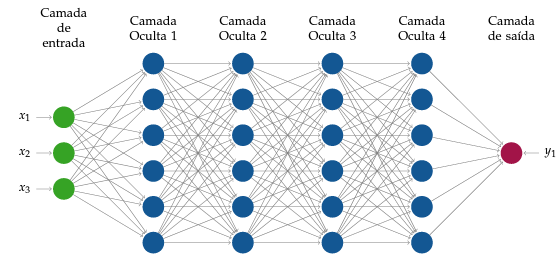
\includegraphics[scale=0.8]{imagens/arquitetura_redeneural.png}
    \caption{Arquitetura padrão de um rede neural \textit{feedforward} \cite{izbicki_mendonca2020}}
    \label{fig:arc_cpx_rnp}
    
\end{figure}

Note que as Figuras \ref{fig:arc_smp_rnp} e \ref{fig:arc_cpx_rnp} evidenciam um potencial muito grande de crescimento da rede e naturalmente esse aumento pode acabar gerando um custo computacional elevado quando a rede estiver em treinamento.

\vspace{1cm}

\subsubsection{\textit{Forward propagation}}

O processo \textit{Forward propagation} (ou propagação direta) é o responsável por transmitir as informações, desde a camada de entrada, passando pelas camadas ocultas, até chegar na camada de saída. O \textit{Forward propagation} utiliza da generalização a Equação \ref{neuronio} para cada neurônio presente nas camadas internas da rede neural. Por isso temos que, para cada j-ésimo neurônio, da camada $l$:

\[
z_{j}^{(l)} = b_{j}^{(l)} + \sum_{i=1}^{d_{(l-1)}} w_{ij}a_{i}^{(l-1)} 
\]

\hspace{-1cm}onde:
\begin{itemize}
    \item $w_{ij}$ é o peso associado à conexão entre o neurônio $i$ na camada $l-1$ e o neurônio $i$ na camada $l$;
    \item $a_{(i)}^{(l-1)}$ é a saída do neurônio i na camada anterior $(l-1)$;
    \item $b_{j}^{(l)}$ é o viés (bias) associado ao neurônio j na camada $l$.
\end{itemize}

Logo em seguida é aplicada uma função de ativação $g$ em $z_{i}^{(l)}$ que vai ser a responsável por gerar o resultado final $a_{i}^{(l)}$, do o i-ésimo neurônio na l-ésima camada.

\[a_{i}^{(l)} = g(z_{i}^{(l)})\]

Esse processo vai ser realizado camada a camada, sequencialmente. Logo, supondo que uma rede neural tenha $l$ camadas ocultas e, cada camada contendo $d_l$ neurônios, considerando também $w_{ij}$ como o peso presente no i-ésimo neurônio com a j-ésima saída na camada seguinte ($l+1$), onde $l=0,...,H$. Temos que o resultado final da propagação é igual a:

\begin{equation}
    f(\textbf{x}) = \textbf{a}^{H+1} = g(b_{j}^{(H+1)} + \sum_{i=1}^{d_{H}} w_{ij}a_{i}^{H}) 
\end{equation}


Note que a previsão da rede vem diretamente do resultado obtido da última camada oculta, e esse depende da camada que o antecede e assim sucessivamente até chegar na camada de entrada.


\subsubsection{Função de perda}

Para se obter informações sobre o desempenho do modelo, é escolhida uma função de perda. Uma função bastante utilizada é a do erro do quadrático médio:

\[EQM(f) = \frac{1}{n} \sum_{k=1}^{n} (f(\textbf{x}_k) - y_k)^2\]

Essa função é uma indicadora do quão longe, em média, os valores preditos estão distantes dos valores reais. Note que o resultado da função $f$ depende exclusivamente dos parâmetros da rede (viés e pesos), por isso, se essa função de perda tende a 0, significa que  os parâmetros dessa rede alcançaram um ponto mínimo global. Entretanto, devido a complexidade desse modelo, acabam-se escolhidos pontos locais mínimos, que, dependendo do contexto, acabam satisfazendo o objetivo. A Figura \ref{fig:pesos_lossfunc} ilustra esse comportamento:

\begin{figure}[H]
    \centering
    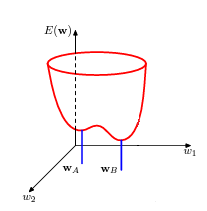
\includegraphics[scale=1]{imagens/pesos_loss_func.png}
    \caption{Comportamentos dos pesos em relação à função de perda. O ponto $w_A$ representa um ponto local mínimo e $w_B$ representa um ponto global mínimo. \cite{bishop2006pattern}}
    \label{fig:pesos_lossfunc}
    
\end{figure}

\subsubsection{\textit{Backpropagation}}

Como a função de perda está relacionada com os parâmetros (\textbf{$\theta$}) da rede, para se minimizar a função de perda R(\textbf{$\theta$}), é necessário encontrar os valores de \textbf{$\theta$} que resolvam esse problema de otimização. Para fazer isso, é necessário calcular o gradiente de  R(\textbf{$\theta$}) em relação à \textbf{$\theta$} \cite{james2013introduction}, 

\begin{equation}
\nabla R(\theta) = \frac{\partial R(\theta)}{\partial \theta}     
\label{gradiente}
\end{equation}


A rede neural, durante todo o treinamento, aplica esse processo do cálculo do gradiente de R(\textbf{$\theta$}) em relação à \textbf{$\theta$}. Esse é um processo iterativo, com o objetivo de mudar o valor de $\theta$ afim de conseguir minimizar a função de perda. Com isso a Equação \ref{gradiente} pode ser descrita nesse processo iterativo como:

\[
\nabla R(\theta^m) = \frac{\partial R(\theta)}{\partial \theta} \bigg\rvert_{\theta = \theta^m},
\]

\hspace{-1.5cm}onde $\theta = \theta_m$ significa que o cálculo do gradiente está sendo realizado na iteração $m$.

E, para conseguir atualizar esse $\theta$, conforme é calculado o gradiente durante as iterações, é utilizada a técnica de gradiente descendente, que pode ser descrita como: 

\[
\theta^{m+1} \leftarrow \theta^{m} - \lambda\frac{\partial R(\theta^m)}{\partial \theta^m}
\]

\hspace{-1.5cm}sendo $\lambda$ o parâmetro que vai definir a magnitude de influência da derivada  $\frac{\partial R(\theta^m)}{\partial \theta^m}$ em $\theta^{m}$.

\begin{figure}[H]
    \centering
    \caption{Representação do método do gradiente descendente para a estimação de um parâmetro.}
    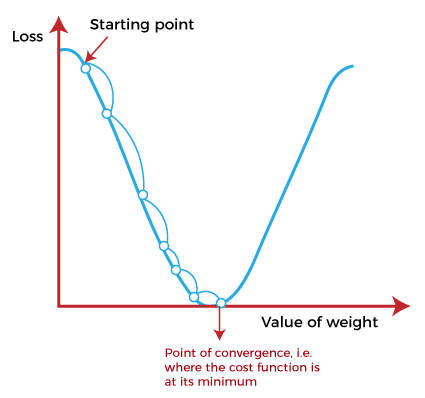
\includegraphics[scale=0.7]{imagens/gradient_descent.png}
    \caption*{Fonte: https://www.javatpoint.com/gradient-descent-in-machine-learning}
    \label{fig:gradient_descent}
    
\end{figure}

A Figura \ref{fig:gradient_descent} demonstra o processo do gradiente descendente. Os parâmetros são iniciados com algum valor e, conforme ocorre os processos iterativos de aprendizado, o parâmetro converge para um mínimo da função de perda. Note que a distância entre cada ponto é definida pelo $\lambda$ ou taxa de aprendizado.


Todo esse processo é realizado em cada parâmetro que existe na rede neural. Assim como as informações das variáveis são passadas camada a camada, saindo da camada de entrada, passando pelas camadas ocultas e chegando na camada de saída, visto anteriormente como \textit{Forward propagation}, a informação do resultado da rede na função de perda é passada de forma contrária. O gradiente de cada parâmetro é calculado primeiro nas camadas mais próximas da saída, e essa informação é repassada para trás, chegando até os parâmetros próximos aos da camada de entrada. Esse processo é chamado de \textit{Backpropagation} \cite{werbos1974beyond}.


\subsection{SHAP}

A estrutura de uma rede neural, por mais que proporcione bons resultados, mostra uma deficiência na parte interpretativa. Conhecida por ser uma "caixa-preta" pelo fato de sua estrutura ser muito complexa, existe a necessidade de se entender as predições feitas.
Para isso, existem técnicas que abordam o tema de interpretação de modelos de redes neurais e dentro delas existe a técnica SHAP, que através dela é possível entender como as variáveis de entrada influenciam as previsões do modelo, fornecendo \textit{insights} sobre sua lógica e permitindo uma explicação clara e confiável. Isso contribui para a transparência, confiabilidade e aceitação dos modelos, além de auxiliar na detecção de viéses e discriminação. 

\subsubsection{Valores de Shapley}

Os valores de Shapley foram
desenvolvidos por Lloyd Shapley \cite{shapley1953value} no contexto da teoria de jogos, e essa técnica ganhou   força na área de inteligência artificial pela sua capacidade de conseguir interpretar modelos preditivos tidos como "caixa-preta". No método criado por Shapley, existiam uma quantidade de jogadores que exerciam juntos determinada atividade, e o intuito era observar o ganho que um jogador (ou um conjunto de jogadores), obtinha ao ser adicionado para realizar a mesma tarefa, sem a presença do restante do grupo. 

Podemos definir \textbf{F} como o conjunto de jogadores (ou as variáveis explicativas) presentes na atividade, logo $\textbf{F} = \{1,2,..., \textbf{M}\}$, onde \textbf{M} é o número de variáveis.
Definindo \textbf{S} como uma coligação do conjunto \textbf{F} $(\textbf{S} \subseteq \textbf{F})$, temos, por exemplo, as seguintes possibilidades de \textbf{S}, quando \textbf{M} é igual a 3:

$$ \{\{\emptyset\},\{1\},\{2\},\{3\},\{1,2\},\{1,3\},\{2,3\},\{1,2,3\}\}$$

Podemos definir também $\nu$ como uma função que vai mapear um conjunto de valores e retornar um número real. Com isso, o retorno de $\nu(\textbf{S})$ é um número real que pode ser definido como 
o "trabalho da coligação \textbf{S} ". Esse valor é equivalente ao total ganho que os jogadores podem obter caso trabalhem juntos em uma determinada coligação.

Para calcular o ganho ao adicionar uma variável $i$ ou a importância do jogador em específico, pode-se calcular o ganho quando é adicionada aquela variável na coligação menos a coligação sem a adição daquela variável, ficando da seguinte maneira:

\[
\nu({\textbf{S} \cup \{i\})} - \nu({\textbf{S})}  
\]

No exemplo acima, caso queiramos calcular o efeito da coligação \{3\}, poderíamos fazer:

\[
Contribuição \hspace{1mm} de \hspace{1mm} \{3\} = \nu(\{1,2,3\}) - \nu(\{1,2\})  
\]

Mas suponha que as variáveis (ou jogadores) \{2\} e \{3\} sejam extremamente semelhantes. Quando é calculado o ganho após inserir \{2\} na coligação \{1,2\}, é possível notar um aumento substancial, mas quando é adicionado \{3\} na coligação \{1,2,3\}, o ganho obtido é muito pouco. Como as variáveis exercem um papel parecido, o ganho maior ficou sujeito à variável que foi adicionada primeiro na coligação, não necessariamente porque uma é mais importante que a outra. 
Por isso, para calcular o real ganho da variável \{i\}, é necessário testar todas as permutações de \textbf{F} (conjunto de jogadores) e obter a contribuição de \{i\} em cada uma delas, para então fazer a média dessas contribuições. Por exemplo, definindo \textbf{F} = \{1,2,3,4\}, suponha que estamos interessados em calcular a contribuição de \{3\}, logo, podemos obter a seguinte permutação de  \textbf{F}:

$$[3,1,2,4]$$

Calculando a contribuição de \{3\}, temos: 

$$\nu(\{3\}) - \nu(\emptyset) $$

Outra permutação poderia ser :

$$[2,4,3,1]$$

Calculando a contribuição de \{3\}, nessa permutação temos: 

$$\nu(coligação \hspace{1mm} de \hspace{1mm} [2,4,3]) - coligação \hspace{1mm} de \hspace{1mm} [2,4]) $$

Uma observação deve ser feita: a função $\nu$ considera a coligação como argumento, não a permutação. A coligação é um conjunto, com isso a ordem dos elementos não importa, mas a permutação é uma coleção ordenada de elementos. Na permutação do tipo [3,1,2,4], 3 é a primeira variável adicionada e 4 é a última. Por isso, para cada permutação a ordem dos elementos pode mudar a contribuição do total ganho, contudo o total ganho da permutação somente depende dos elementos, não da ordem. Logo:

\[\nu(coligação \hspace{1mm} de \hspace{1mm} [3,1,2,4]) = \nu(\{1,4,2,3\})\]

Sendo assim, para cada permutação \textbf{P}, é preciso primeiro calcular o ganho da coligação das variáveis que foram adicionadas antes de \{i\}, e esse conjunto pode ser chamado de coligação \textbf{S}. Feito isso, agora é preciso calcular o ganho das coligações que são formadas ao adicionar \{i\} em \textbf{S}, e podemos chamar isso de $\textbf{S} \cup \{i\}$. Com isso, a contribuição da variável \{i\}, denotada por $\phi_{i}$, é:

\begin{equation}
 \phi_i = \frac{1}{|\textbf{F}|!}\sum_{\textbf{P}} [\nu(\textbf{S}\cup\{i\}) - \nu(\textbf{S})]
 \label{eq:value_shap_ini}
\end{equation}

O número total de permutações de \textbf{F} é $|\textbf{F}|!$. Logo, podemos dividir a soma das contribuições por $|\textbf{F}|!$ para encontrar o valor esperado de contribuição de \{i\}. A Figura \ref{fig:total_permuts_shap} mostra como é feito esse calculo para um determinado jogador $\{i\}$.

\begin{figure}[H]
    \centering
    \caption{Ganho do jogador 3 em relação à todas as permutações de jogadores.}
    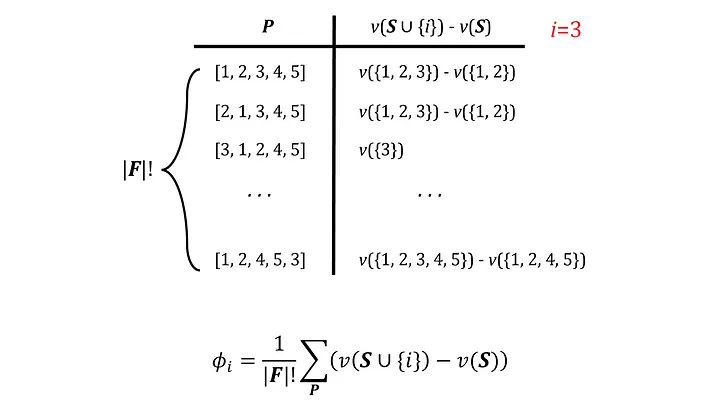
\includegraphics[scale=0.5]{imagens/shap.png}
    \caption*{Fonte: https://towardsdatascience.com/introduction-to-shap-values-and-their-application-in-machine-learning-8003718e6827}
    \label{fig:total_permuts_shap}
    
\end{figure}

É possível perceber que algumas permutações possuem a mesma contribuição, desde que suas coligações 
$\textbf{S}\cup\{i\}$ e \textbf{S} sejam as mesmas. Com isso, para reduzir o processo do cálculo de contribuição de cada permutação, pode-se identificar quantas vezes a permutação gerada vai resultar em uma contribuição que seja igual a outra.


Para fazer isso, é necessário descobrir quantas permutações podem ser formadas de cada coligação. Podemos definir $\textbf{F} - \{i\}$ como o conjunto de todas as variáveis excluindo a variável \{i\}, e \textbf{S} como uma das coligações de $\textbf{F} - \{i\}$ (\textbf{S} \subseteq  $\textbf{F} - \{i\}$ ).

Logo, para cada coligação \textbf{S} temos $|\textbf{S}|!$ possíveis permutações, que corresponde às possibilidades  de variáveis e suas respectivas ordens antes de adicionar a variável \{i\}.

Tendo os conjuntos $\textbf{S}\cup\{i\}$ e \textbf{S} definidos, resta agora achar as possíveis permutações das variáveis restantes. E para saber o valor restante é preciso calcular o tamanho do conjunto gerado por: \textbf{F} - ($\textbf{S}\cup\{i\}$ + 1)
que basicamente é o que resta das variáveis para completar o conjunto \textbf{F}.

A Figura \ref{fig:permut_e_colig}  mostra o que acontece quando se escolhe o jogador $i$, nesse caso $i=3$. Note que, na linha das coligações, é definido as possíveis coligações de \textbf{S}, que seria as permutações dos jogadores 1 e 2, temos a coligação de um único elemento na coluna $\{i\}$, que sempre vai ser o próprio elemento, em seguida a coligação dos jogadores restantes. Na linha das permutações é definida todas as possíveis permutações para \textbf{S}, para $\{i\}$ e para $\textbf{F}-\textbf{S}-\{i\}$. E na última linha é representado o tamanho do conjunto formado pela permutação/coligação descrita anteriormente.

\begin{figure}[H]
    \centering
    \caption{Relação entre permutações e coalizões.}
    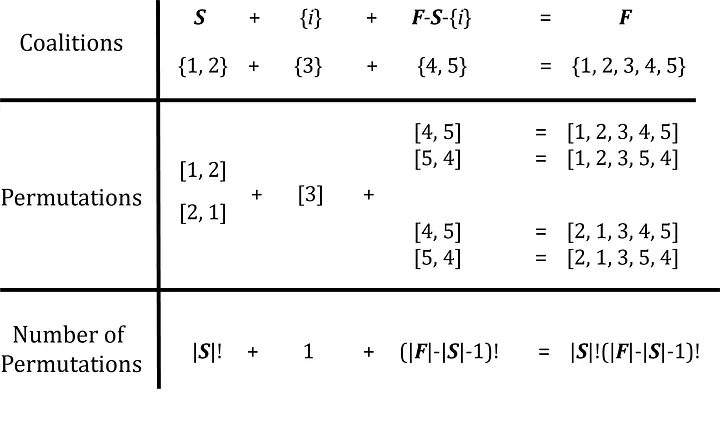
\includegraphics[scale=0.5]{imagens/shap1.png}
    \caption*{Fonte: https://towardsdatascience.com/introduction-to-shap-values-and-their-application-in-machine-learning-8003718e6827}
    \label{fig:permut_e_colig}
    
\end{figure}

Com isso, podemos reescrever a Equação \ref{eq:value_shap_ini} da seguinte maneira:

\[
\phi_i= 
\sum_{\textbf{S} \subseteq  \textbf{F} - \{i\}}
\frac{|\textbf{S}|!(|\textbf{F}| - |\textbf{S}| - 1)!}{|\textbf{F}|!}
[\nu(\textbf{S}\cup\{i\}) - \nu(\textbf{\textbf{S}})],
\]
\hspace{1.5cm} onde $\phi_i$ é o valor de shapley para a variável \{i\}.

\subsubsection{Shapley Additive Explanations}

Fazendo a relação do valor de Shapley para o SHAP (Shapley Additive Explanations), temos que a função característica $\nu$ é equivalente à função $f(x)$ responsável por fazer as predições. E os valores de SHAP são calculados a partir das observações que entram no modelo. Com isso, a fórmula do valor de SHAP, para cada conjunto de observação e variável especificada, se dá por:

\[
\phi_i(f,\textbf{x})= 
\sum_{\textbf{S} \subseteq  \textbf{F} - \{i\}}
\frac{|\textbf{S}|!(|\textbf{F}| - |\textbf{S}| - 1)!}{|\textbf{F}|!}
[f_{\textbf{S}\cup\{i\}}(\textbf{x}_{\textbf{S}\cup\{i\}}) - f_{\textbf{S}}(\textbf{x}_{\textbf{S}})
]
\]

Perceba que $f_\textbf{S}(\textbf{x}_S)$ representa o resultado do modelo com somente as variáveis que estão na coligação $\textbf{S}$, algo que na realidade não é permitido na maioria dos modelos. Por isso, uma aproximação desse resultado é a seguinte:

\begin{equation}    
f_S(\textbf{x}_S)) \approx E[f(\textbf{x}|\textbf{x}_S)] \approx 
\frac{1}{k} \sum_{i=1}^{k}
f(\textbf{x}_{\bar{S}}^{(i)}, \textbf{x}_S)
\label{eq:SHAP_detalhado}
\end{equation}


\begin{figure}[H]
    \centering
    \caption{Cálculo de $f_{\textbf{S}}$, sendo S o conjunto de variáveis $X_1, X_3, X_4$, dentre as observações de um conjunto de dados.}
    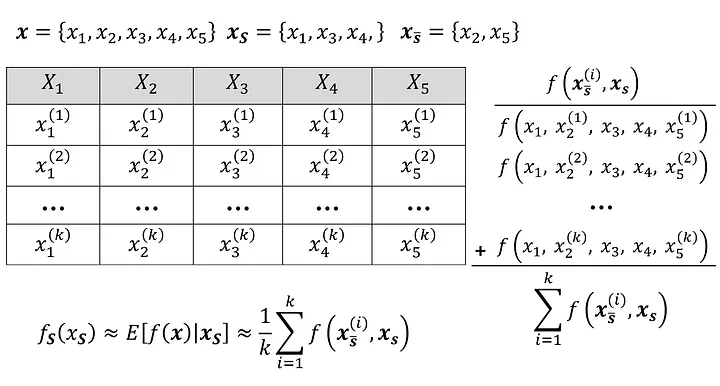
\includegraphics[scale=0.5]{imagens/shap_explicado.png}
    \caption*{Fonte: https://towardsdatascience.com/introduction-to-shap-values-and-their-application-in-machine-learning-8003718e6827}
    \label{fig:calculo_esforço}

    
\end{figure}
A Figura \ref{fig:calculo_esforço} representa, para cada observação do conjunto de dados, a Equação \ref{eq:SHAP_detalhado}. Neste caso, as variáveis $X_1, X_3$ e $ X_4$ representam o conjunto $\textbf{S}$, e escolhendo um valor $x_1, x_3$ e $ x_4$ dessas variáveis, respectivamente, calcula-se $f$ para cada observação do conjunto de dados, travando $x_1, x_3$ e $ x_4$ na função e utilizando o valor das variáveis complementares, que neste caso são os valores de $X_2$ e $X_5$, em suas respectivas observações. Feito isso, é calculada média desses valores que corresponde justamente com o resultado da função $f_{\textbf{S}}(x_{\textbf{S}})$.